\documentclass[journal,12pt,onecolumn]{IEEEtran}
\usepackage{graphicx, float}
\graphicspath{{Figs/}}
\usepackage{multicol}
\usepackage{parskip}
\usepackage{titlesec}
\usepackage{color}
\usepackage{enumitem}
\usepackage{amsmath,amssymb,amsfonts,amsthm}
\usepackage{array}
\usepackage{booktabs}
\usepackage[table]{xcolor}
\usepackage{longtable}
\usepackage{gensymb}
\usepackage{cite}
\usepackage{algorithmic}
\usepackage{textcomp}
\usepackage{txfonts}
\usepackage{listings}
\usepackage{mathtools}
\usepackage{comment}
\usepackage{tkz-euclide}
\usepackage[breaklinks=true]{hyperref}
\usepackage{gvv}
\usepackage{gvv-book}
\usepackage[latin1]{inputenc}
\usetikzlibrary{arrows.meta, positioning}
\usepackage{xparse}
\usepackage{calc}
\usepackage{multirow}
\usepackage{hhline}
\usepackage{ifthen}
\usepackage{lscape}
\usepackage{tabularx}
\usepackage{circuitikz}
\usepackage{tikz}
\newcommand{\BEQA}{\begin{eqnarray}}
\newcommand{\EEQA}{\end{eqnarray}}
\theoremstyle{remark}
\title{GE 2022: Geomatics Engineering}
\author{EE25BTECH11064 - Yojit Manral}

\begin{document}

\maketitle

\begin{enumerate}

\item Writing too many things on the \makebox[1cm]{\hrulefill} while teaching could make the students get \makebox[1cm]{\hrulefill}.

\hfill (GATE GE 2022)

\begin{enumerate}
\begin{multicols}{2}
    \item bored / board
    \item board / bored
    \item board / board
    \item bored / bored
\end{multicols}
\end{enumerate}

\item Which one of the following is a representation (not to scale and in bold) of all values of $x$ satisfying the inequality $2 - 5x \leq -\frac{6x - 5}{3}$ on the real number line?

\hfill (GATE GE 2022)

\begin{enumerate}
\begin{multicols}{2}
    \item
    \begin{minipage}{\linewidth}
        \centering
        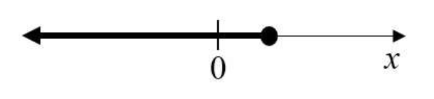
\includegraphics[width=0.9\columnwidth]{figs/fig_2.1.png}
        \label{fig:option2.1}
    \end{minipage}
    \item
    \begin{minipage}{\linewidth}
        \centering
        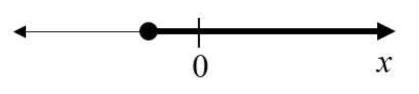
\includegraphics[width=0.9\columnwidth]{figs/fig_2.2.png}
        \label{fig:option2.2}
    \end{minipage}
    \item
    \begin{minipage}{\linewidth}
        \centering
        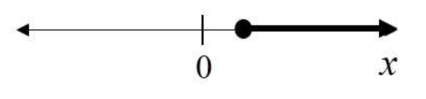
\includegraphics[width=0.9\columnwidth]{figs/fig_2.3.png}
        \label{fig:option2.3}
    \end{minipage}
    \item
    \begin{minipage}{\linewidth}
        \centering
        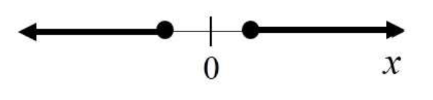
\includegraphics[width=0.9\columnwidth]{figs/fig_2.4.png}
        \label{fig:option2.4}
    \end{minipage}
\end{multicols}
\end{enumerate}

\item If $f(x) = 2 \ln(\sqrt{e^x})$, what is the area bounded by $f(x)$ for the interval $[0, 2]$ on the $x$-axis?

\hfill (GATE GE 2022)

\begin{enumerate}
\begin{multicols}{4}
    \item $\frac{1}{2}$
    \item $1$
    \item $2$
    \item $4$
\end{multicols}
\end{enumerate}

\item A person was born on the fifth Monday of February in a particular year. Which one of the following statements is correct based on the above information?

\hfill (GATE GE 2022)

\begin{enumerate}
    \item The 2nd February of that year is a Tuesday
    \item There will be five Sundays in February in that year
    \item The 1st February of that year is a Sunday
    \item All Mondays of February in that year have even dates
\end{enumerate}

\item
\begin{figure}[H]
    \centering
    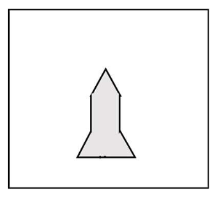
\includegraphics[width=0.3\columnwidth]{figs/fig_5.png}
    \label{fig:question5}
    \caption*{Figure.Q5}
\end{figure}
Which one of the groups given below can be assembled to get the shape that is shown above using each piece only once without overlapping with each other? (rotation and translation operations may be used).

\hfill (GATE GE 2022)

\begin{enumerate}
\begin{multicols}{4}
    \item \begin{minipage}{\linewidth}
        \centering
        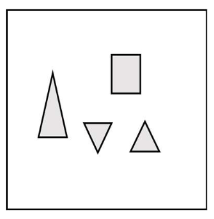
\includegraphics[width=0.9\columnwidth]{figs/fig_5.1.png}
        \label{fig:option5.1}
    \end{minipage}
    \item \begin{minipage}{\linewidth}
        \centering
        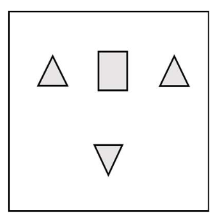
\includegraphics[width=0.9\columnwidth]{figs/fig_5.2.png}
        \label{fig:option5.2}
    \end{minipage}
    \item \begin{minipage}{\linewidth}
        \centering
        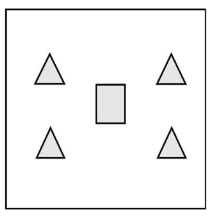
\includegraphics[width=0.9\columnwidth]{figs/fig_5.3.png}
        \label{fig:option5.3}
    \end{minipage}
    \item \begin{minipage}{\linewidth}
        \centering
        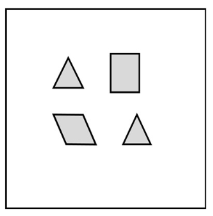
\includegraphics[width=0.9\columnwidth]{figs/fig_5.4.png}
        \label{fig:option5.4}
    \end{minipage}
\end{multicols}
\end{enumerate}

\item Fish belonging to species S in the deep sea have ultra-black skin that are extremely black (ultra-black skin). This helps them not only to avoid predators but also sneakily attack their prey. However, having this extra layer of black pigment results in lower collagen on their skin, making their skin more fragile. \\
Which one of the following is the CORRECT logical inference based on the information in the above passage?

\hfill (GATE GE 2022)

\begin{enumerate}
    \item Having ultra-black skin is only advantageous to species S
    \item Species S with lower collagen in their skin are at an advantage because it helps them avoid predators
    \item Having ultra-black skin has both advantages and disadvantages to species S
    \item Having ultra-black skin is only disadvantageous to species S but advantageous only to their predators
\end{enumerate}

\item For the past $m$ days, the average daily production was 100 units/day. If today's production of 180 units changes the average to 110 units/day, what is the value of $m$?

\hfill (GATE GE 2022)

\begin{enumerate}
\begin{multicols}{4}
    \item 18
    \item 10
    \item 7
    \item 5
\end{multicols}
\end{enumerate}

\item Consider the following functions for non-zero positive integers, $p$ and $q$.
\begin{figure}[H]
    \centering
    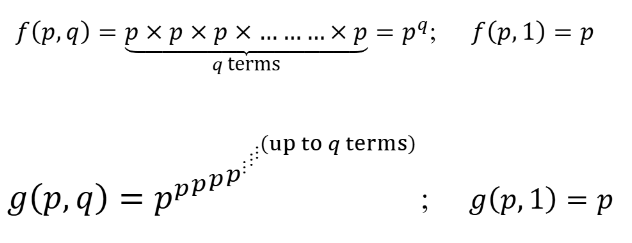
\includegraphics[width=0.6\columnwidth]{figs/fig_8.png}
    \label{fig:question8}
    \caption*{Figure.Q8}
\end{figure}
Which one of the following options is correct based on the above?

\hfill (GATE GE 2022)

\begin{enumerate}
\begin{multicols}{2}
    \item $f(2,2) = g(2,2)$
    \item $f(g(2,2), 2) < f(2, g(2,2))$
    \item $g(2,1) \ne f(2,1)$
    \item $f(3,2) > g(3,2)$
\end{multicols}
\end{enumerate}

\item Four cities P, Q, R, S are connected through one-way routes as shown in the figure. The travel time between any two connected cities is one hour. The boxes beside each city name describe the starting time of first train of the day and their frequency of operation. For example, from city P, the first trains of the day start at 8 AM with a frequency of 90 minutes to each of R and S. A person does not spend additional time at any city other than the waiting time for the next connecting train. \\
If the person starts from R at 7 AM, visits S and returns to R, what is the minimum time required?
\begin{figure}[H]
    \centering
    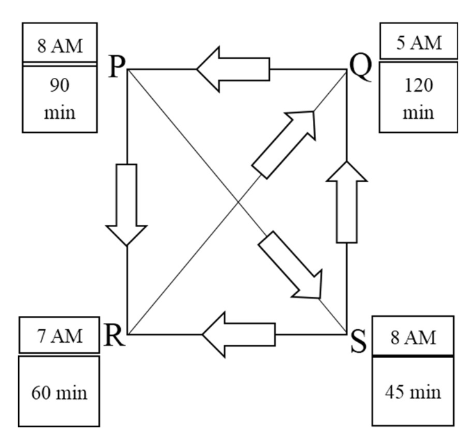
\includegraphics[width=0.4\columnwidth]{figs/fig_9.png}
    \label{fig:question9}
    \caption*{Figure.Q9}
\end{figure}

\hfill (GATE GE 2022)

\begin{enumerate}
\begin{multicols}{2}
    \item 6 hours 30 minutes
    \item 3 hours 45 minutes
    \item 4 hours 30 minutes
    \item 5 hours 15 minutes
\end{multicols}
\end{enumerate}

\item Equal sized circular regions are shaded in a square sheet of side 1 cm side length. Two cases, case M and case N, are considered as shown in the figures below. In the case M, four circles are shaded in the square sheet and in the case N, nine circles are shaded in the square sheet as shown. \\
What is the ratio of the unshaded regions (M:N)?
\begin{figure}[H]
    \centering
    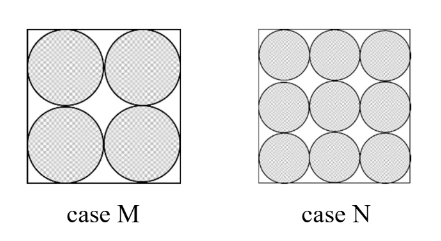
\includegraphics[width=0.4\columnwidth]{figs/fig_10.png}
    \label{fig:question10}
    \caption*{Figure.Q10}
\end{figure}

\hfill (GATE GE 2022)

\begin{enumerate}
\begin{multicols}{4}
    \item 2:3
    \item 1:1
    \item 3:2
    \item 2:1
\end{multicols}
\end{enumerate}

\textbf{PART A: Common FOR ALL CANDIDATES}

\item Most probable value of a quantity:

\hfill (GATE GE 2022)

\begin{enumerate}
    \item always increases with increase in True value
    \item always decreases with decrease in True value
    \item is always equal to True value
    \item is nearest to True value
\end{enumerate}

\item Two surveyors P and Q measured a 20 m distance six times each, as given below(in m).
\begin{align*}
    Surveyor P &: 19.97, 20.02, 20.04, 19.98, 19.96, 20.03 \\
    Surveyor Q &: 20.05, 20.07, 20.05, 20.06, 20.07, 20.07
\end{align*}
On the basis of accuracy and precision of the measured values, choose the CORRECT statement.

\hfill (GATE GE 2022)

\begin{enumerate}
    \item Observed values of Surveyor P are less precise and observed values of Surveyor Q are more accurate. 
    \item Observed values of Surveyor P are more precise and observed values of Surveyor Q are less accurate.
    \item Observed values of Surveyor P are more accurate and observed values of Surveyor Q are more precise.
    \item Observed values of Surveyor P are less accurate and observed values of Surveyor Q are less precise.
\end{enumerate}

\item Identify the error, which has all the following characteristics:
\begin{enumerate}[label=\arabic*)]
\item Caused by observer's misunderstanding and carelessness 
\item Reading an angle counter-clockwise, but recording it as clockwise angle 
\item Sighting the wrong target 
\item Poor judgment by the observer 
\end{enumerate}

\hfill (GATE GE 2022)

\begin{enumerate}
\begin{multicols}{2}
    \item Mistake
    \item Cumulative error
    \item Probable error
    \item Accidental error
\end{multicols}
\end{enumerate}

\item Electromagnetic Spectrum can be broadly divided as (in order of increasing wavelength):

\hfill (GATE GE 2022)

\begin{enumerate}
    \item X-rays, Gamma rays, Infrared, Ultraviolet, Visible, Radiowave, Microwave
    \item Gamma rays, X-rays, Radiowave, Microwave, Ultraviolet, Infrared, Visible
    \item X-rays, Gamma rays, Microwave, Radiowave, Ultraviolet, Infrared, Visible
    \item Gamma rays, X-rays, Ultraviolet, Visible, Infrared, Microwave, Radiowave
\end{enumerate}

\item Relationship between wavelength ($\lambda$), frequency ($\nu$), and velocity ($c$) of EM waves is:

\hfill (GATE GE 2022)

\begin{enumerate}
\begin{multicols}{4}
    \item $c = \nu^2 / \lambda$
    \item $c = \nu / \lambda$
    \item $c = \nu \lambda$
    \item $c = \nu \lambda^2$
\end{multicols}
\end{enumerate}

\item Spectral signature of an object in a satellite image does NOT depend on:

\hfill (GATE GE 2022)

\begin{enumerate}
\begin{multicols}{2}
    \item season of the year
    \item wavelength of EM spectrum
    \item swath width of the satellite
    \item reflectance value from the object
\end{multicols}
\end{enumerate}

\item Component of GPS signal deciphered by all types of GPS receivers is:

\hfill (GATE GE 2022)

\begin{enumerate}
\begin{multicols}{2}
    \item Coarse-Acquisition code
    \item Precision code
    \item Link-1 frequency
    \item Link-2C frequency
\end{multicols}
\end{enumerate}

\item For 3D-positioning, GLobal Navigational Satellite System (GNSS) requires a minimum of \makebox[1cm]{\hrulefill} satellites.

\hfill (GATE GE 2022)

\begin{enumerate}
\begin{multicols}{4}
    \item 3
    \item 4
    \item 5
    \item 2
\end{multicols}
\end{enumerate}

\item Basic objective of NAVSTAR GPS is to provide services for:

\hfill (GATE GE 2022)

\begin{enumerate}
\begin{multicols}{2}
    \item Positioning, Velocity and Timing
    \item Positioning, Navigation and Timing
    \item Velocity, Navigation and Timing
    \item Positioning, Velocity and Navigation
\end{multicols}
\end{enumerate}

\item A satellite image with 6-bit radiometric resolution has \makebox[1cm]{\hrulefill} gray levels.

\hfill (GATE GE 2022)

\begin{enumerate}
\begin{multicols}{4}
    \item 16
    \item 32
    \item 64
    \item 128
\end{multicols}
\end{enumerate}

\item Thermal Infrared images are provided by

\hfill (GATE GE 2022)

\begin{enumerate}
\begin{multicols}{2}
    \item LANDSAT MSS and IRS LISS-II sensors
    \item SPOT and CARTOSAT
    \item IKONOS and QUICKBIRD
    \item LANDSAT TM and NOAA AVHRR sensors
\end{multicols}
\end{enumerate}

\item Which of the following gets mitigated in DGPS positioning?

\hfill (GATE GE 2022)

\begin{enumerate}
\begin{multicols}{4}
    \item Atmospheric error
    \item Multi-path error
    \item Cycle-slip error
    \item Topographic error
\end{multicols}
\end{enumerate}

\item In GIS database, which type of attribute may be used to represent area?

\hfill (GATE GE 2022)

\begin{enumerate}
\begin{multicols}{4}
    \item Nominal
    \item Interval
    \item Ratio
    \item Ordinal
\end{multicols}
\end{enumerate}

\item What is attribute uncertainty?

\hfill (GATE GE 2022)

\begin{enumerate}
    \item Error due to imprecision in coordinate registration
    \item Error due to incorrect labelling or quantification of features
    \item Error in the source document due to cartographic bias
    \item Error associated with displacement of the object from its true location
\end{enumerate}

\item In GIS, \makebox[2cm]{\hrulefill} triangulation is a proximal method that satisfies the requirement that a circle drawn through the three nodes of a triangle contains no other node.

\hfill (GATE GE 2022)

\begin{enumerate}
\begin{multicols}{4}
    \item Dalhousie
    \item Delaunay
    \item David
    \item Davenport
\end{multicols}
\end{enumerate}

\item In GIS, reclassification is performed to

\hfill (GATE GE 2022)

\begin{enumerate}
    \item group ranges of values into a single value within a data layer
    \item segment a data layer into multiple data layers
    \item combine multiple data layers to a single data layer
    \item classify a data layer using many attributes
\end{enumerate}

\item For the following observation equation:
\begin{align*}
2\alpha &= 124^\circ 52' 22''\hspace{2cm}(weight 4),
\end{align*}
the weight of $\frac{\alpha}{3}$ is \makebox[1cm]{\hrulefill} (in integer).

\hfill (GATE GE 2022)

\item Following observation equations are obtained in a survey task:
\begin{align*}
x + y &= 3 \\
2x + y &= 6 \\
x + 2y &= 4
\end{align*}
Using least square method, the most probable values of $x$ and $y$ will be:

\hfill (GATE GE 2022)

\begin{enumerate}
\begin{multicols}{2}
    \item $x = 2.10, y = 0.90$
    \item $x = 2.64, y = 0.64$
    \item $x = 2.51, y = 0.51$
    \item $x = 2.75, y = 0.75$
\end{multicols}
\end{enumerate}

\item The internal angles P, Q, R of a triangle are observed in degree minute second ($^\circ$ $'$ $''$) using a Total Station. The angles along with their probable errors are given below:
\begin{align*}
P &= 40^\circ 30' 01'' \pm 02'' \\
Q &= 60^\circ 00' 02'' \pm 03'' \\
R &= 79^\circ 30' 05'' \pm 04''
\end{align*}
The corrected values of the angles P, Q and R are:

\hfill (GATE GE 2022)

\begin{enumerate}
    \item P = $40^\circ 30' 01''$, Q = $60^\circ 00' 02''$, R = $79^\circ 30' 05''$
    \item P = $40^\circ 29' 59.6''$, Q = $59^\circ 59' 59.5''$, R = $79^\circ 30' 0.9''$
    \item P = $40^\circ 29' 59.9''$, Q = $59^\circ 59' 59.5''$, R = $79^\circ 30' 0.6''$
    \item P = $40^\circ 29' 59''$, Q = $59^\circ 59' 59''$, R = $79^\circ 30' 02''$
\end{enumerate}

\item How many number of cells of a 30 m spatial resolution DEM would be required to cover a 1:50,000 topographic map of Survey of India, assuming that 1 minute = 1.85 km?

\hfill (GATE GE 2022)

\begin{enumerate}
\begin{multicols}{4}
    \item 855,625
    \item 855,525
    \item 855,425
    \item 855,325
\end{multicols}
\end{enumerate}

\item Choose the CORRECT statement(s):

\hfill (GATE GE 2022)

\begin{enumerate}
    \item True Color Composite is produced by superimposing Red band in Red, Green band in Green, and Blue band in Blue color.
    \item True Color Composite is produced by superimposing Blue band in Red, Green band in Green, and Red band in Blue color.
    \item Standard False Color Composite is produced by superimposing Near Infrared band in Red, Red band in Green, and Green band in Blue color.
    \item Standard False Color Composite is produced by superimposing Green band in Red, Green band in Green, and Near Infrared band in Blue color.
\end{enumerate}

\item Choose the CORRECT statement(s) in case of visual image interpretation:

\hfill (GATE GE 2022)

\begin{enumerate}
    \item Tone/Color is a primary element while Size, Shape and Texture are secondary elements.
    \item Size, Shape and Texture are primary elements while Tone/Color is a secondary element.
    \item Texture refers to the frequency of tonal changes in an area of image.
    \item Tone/Color is a primary element while Pattern and Association are secondary elements.
\end{enumerate}

\item The spatial resolution of a satellite image \textbf{P} is 80 m and another satellite image \textbf{Q} is 20 m; each of 512 $\times$ 512 pixel size. Choose the CORRECT option(s):

\hfill (GATE GE 2022)

\begin{enumerate}
    \item Image P will cover four times the area of image Q.
    \item Image P will cover sixteen times the area of image Q.
    \item Minor details will be more clear in image Q as compared to image P.
    \item Image P is higher resolution and image Q is lower resolution.
\end{enumerate}

\item Which statement(s) is/are CORRECT for Hyperspectral images?

\hfill (GATE GE 2022)

\begin{enumerate}
\begin{multicols}{2}
    \item Bandwidth is large.
    \item Bandwidth is narrow.
    \item Number of bands are more.
    \item Bands are contiguous.
\end{multicols}
\end{enumerate}

\item Satellite-Based NAVSTAR GPS Augmentation System(s) is/are:

\hfill (GATE GE 2022)

\begin{enumerate}
\begin{multicols}{4}
    \item EGNOS
    \item WAAS
    \item GAGAN
    \item DGPS
\end{multicols}
\end{enumerate}

\item Identify the CORRECT statement(s):

\hfill (GATE GE 2022)

\begin{enumerate}
    \item NAVSTAR GPS consists of minimum 24 satellites.
    \item Precision of GPS positioning is being defined by its standard deviation.
    \item DGPS method provides more accurate 3D-position than Relative Static post-processing method.
    \item GPS observations from geodetic GPS receiver provide less accurate position than GPS code receiver.
\end{enumerate}

\item Identify the CORRECT statement(s):

\hfill (GATE GE 2022)

\begin{enumerate}
    \item For accurate GPS positioning, Geometric Dilution of Precision should be as large as possible.
    \item Integer ambiguity is associated with carrier frequency observation of GPS signal.
    \item GPS is one way ranging system for user.
    \item GPS is two way ranging system for user.
\end{enumerate}

\item During GPS Surveying, initialization of rover receiver is required for:

\hfill (GATE GE 2022)

\begin{enumerate}
\begin{multicols}{2}
    \item Relative Static method
    \item Relative Kinematic method
    \item Stop and Go method
    \item Kinematic On Fly method
\end{multicols}
\end{enumerate}

\item Centroid of a polygon is:

\hfill (GATE GE 2022)

\begin{enumerate}
    \item geometric center of the polygon
    \item arithmetic mean position of all its vertices in two coordinate directions
    \item the point at which a cutout of the polygon could be perfectly balanced on the tip of a pin
    \item center of polyline
\end{enumerate}

\item The area of a buffer of 50 m around a proposed 1 km straight road segment to restrict any future construction is \makebox[1cm]{\hrulefill} sq. m. (in integer). (Take the value of $\pi = 3.14$)

\hfill (GATE GE 2022)

\item The Degree of Accuracy of a traverse having error of closure of 0.5 m and perimeter of 100 m is \makebox[1cm]{\hrulefill} (round off to 3 decimal places).

\hfill (GATE GE 2022)

\item Using the following regression equations, the correlation coefficient between two survey quantities $x$ and $y$ will be \makebox[1cm]{\hrulefill} (round off to 2 decimal places):
\begin{align*}
2x - 5y + 98 &= 0 \\
6x - 7y + 114 &= 0
\end{align*}

\hfill (GATE GE 2022)

\item If population variance is 14.8, sample variance is 15.4 and the number of degrees of freedom is 10, then Chi-square value is \makebox[1cm]{\hrulefill} (round off to 2 decimal places).

\hfill (GATE GE 2022)

\item Height of a station determined by Global Navigational Satellite System (GNSS) is 284.097 m and the geoid height of the station is -30.052 m. The elevation of the station is \makebox[1cm]{\hrulefill} m (round off to 3 decimal places).

\hfill (GATE GE 2022)

\item Number of cells required to cover an area of 9 sq. km of ASTER-GDEM are \makebox[1cm]{\hrulefill} (in integer).

\hfill (GATE GE 2022)

\item If a 1:50,000 scale map is digitized to an accuracy of $\pm$ 0.5 mm, the level of error that might be expected in ground is $\pm$ \makebox[1cm]{\hrulefill} m (in integer).

\hfill (GATE GE 2022)

\textbf{PART B: FOR Section I CANDIDATES ONLY}

\item The main principle of Surveying is to work from

\hfill (GATE GE 2022)

\begin{enumerate}
\begin{multicols}{2}
    \item whole to part
    \item part to whole
    \item higher elevation to lower elevation
    \item lower elevation to higher elevation
\end{multicols}
\end{enumerate}

\item The type of survey carried out to define the property boundaries for transfer of land property is called

\hfill (GATE GE 2022)

\begin{enumerate}
\begin{multicols}{4}
    \item city survey
    \item cadastral survey
    \item municipality survey
    \item geodetic survey
\end{multicols}
\end{enumerate}

\item Departure of a line of a traverse is obtained by multiplying its length by the \makebox[1cm]{\hrulefill} of the reduced bearing of the line.

\hfill (GATE GE 2022)

\begin{enumerate}
\begin{multicols}{4}
    \item Sine
    \item Cosine
    \item Tangent
    \item Cotangent
\end{multicols}
\end{enumerate}

\item The multiplying constant of a Tacheometer, where $f$ is the focal length and $i$ is the distance between the stadia hairs, is

\hfill (GATE GE 2022)

\begin{enumerate}
\begin{multicols}{4}
    \item $i/f$
    \item $f^2 / i$
    \item $f / i$
    \item $f \times i$
\end{multicols}
\end{enumerate}

\item The camera axis of an aerial camera is defined as

\hfill (GATE GE 2022)

\begin{enumerate}
    \item the line joining the optical centres of the objective and eyepiece lens
    \item the perpendicular line between the photographic centre and optical centre of the objective lens
    \item the line passing through the centre of the camera lens and perpendicular to the camera plane and the photo plane
    \item the line perpendicular to the plumb line
\end{enumerate}

\item Bowditch rule for adjusting a closed traverse of perimeter $l$ is based on the assumption that the probable error is proportional to

\hfill (GATE GE 2022)

\begin{enumerate}
\begin{multicols}{4}
    \item $l$
    \item $\sqrt{l}$
    \item $l^2$
    \item $1/\sqrt{l}$
\end{multicols}
\end{enumerate}

\item Select the INCORRECT statement:

\hfill (GATE GE 2022)

\begin{enumerate}
    \item Scale of a tilted photograph is uniform throughout its extent
    \item The relief displacement of any point will be radial from nadir point of the tilted photograph
    \item The bisector of the angle of tilt intersects the tilted photograph at a point known as isocentre
    \item A line perpendicular to the principal line and passing through the isocentre is known as the axis of tilt
\end{enumerate}

\item A topographic map prepared by Survey of India covers 1 degree by 1 degree area on a single map. The minimum ground distance which can be represented on this map is \makebox[1cm]{\hrulefill} m (round off to 2 decimal places).

\hfill (GATE GE 2022)

\item In a closed traverse, the sum of the latitudes is 1.39 m and the sum of the departures is 2.17 m. The Length and Whole Circle Bearing of the closing error are

\hfill (GATE GE 2022)

\begin{enumerate}
    \item Length = 2.57 m, Whole Circle Bearing = $58^\circ$
    \item Length = 2.57 m, Whole Circle Bearing = $57^\circ$
    \item Length = 2.67 m, Whole Circle Bearing = $58^\circ$
    \item Length = 2.67 m, Whole Circle Bearing = $57^\circ$
\end{enumerate}

\item In surveying, an odometer is used for measuring

\hfill (GATE GE 2022)

\begin{enumerate}
\begin{multicols}{4}
    \item azimuth
    \item horizontal angle
    \item vertical angle
    \item distance
\end{multicols}
\end{enumerate}

\item Choose the CORRECT statement(s):

\hfill (GATE GE 2022)

\begin{enumerate}
    \item The spheroid is a mathematical surface of the Earth
    \item Geoid is an equipotential reference surface of the Earth
    \item True shape of the Earth is perfect spheroid
    \item The WGS-84 datum varies from country to country
\end{enumerate}

\item Choose the CORRECT statement(s):

\hfill (GATE GE 2022)

\begin{enumerate}
    \item Latitude of a place varies from 0° to 90° North or South, and Longitude varies from 0° to 180° East or West of Greenwich Meridian
    \item Latitude of a place varies from 0° to 180° East or West of Greenwich Meridian, and Longitude varies from 0° to 90° North or South
    \item Longitude of a point is the angle between the Greenwich Meridian and the meridian passing through that point
    \item Latitude and Longitude of a place are subject to change with time
\end{enumerate}

\item A map projection is

\hfill (GATE GE 2022)

\begin{enumerate}
    \item a systematic representation of latitude and longitude lines on a plane (paper) map
    \item a representation of 3D shape of Earth on 2D plane
    \item dependent on the location of area on the Earth
    \item required for taking theodolite observations of horizontal angles
\end{enumerate}

\hfill (GATE GE 2022)

\item Face Left and Face Right observations using a vernier theodolite will eliminate

\hfill (GATE GE 2022)

\begin{enumerate}
\begin{multicols}{4}
    \item index error
    \item graduation error
    \item eccentricity error
    \item atmospheric error
\end{multicols}
\end{enumerate}

\item The parallax of a point 'a' on a pair of successive overlapping photographs is 73.22 mm and the micrometer reading of a parallax bar of point 'a' is 12.10 mm. Similarly, the micrometer reading of the parallax bar of point 'b' is 9.65 mm, then the parallax of the point 'b' is \makebox[1cm]{\hrulefill} mm (round off to 2 decimal places).

\hfill (GATE GE 2022)

\item The scale of an aerial photograph is 5 mm = 100 m. The size of the photograph is 23 cm $\times$ 23 cm. If the longitudinal overlap is 65\% and sidelap is 20\%, the number of photographs required to cover an area of 12.5 km $\times$ 8 km is \makebox[1cm]{\hrulefill} (in integer). Given that the flight line is along the longer dimension.

\hfill (GATE GE 2022)

\item An instrument is set up at a station P and the angle of depression to a vane, 1.20 m above the foot of the staff held at Q is 5°. The horizontal distance PQ is 300 m. The R.L. of point Q is \makebox[1cm]{\hrulefill} m (round off to 3 decimal places). Given that the staff reading at a BM (Elevation 436.050 m) is 2.865 m.

\hfill (GATE GE 2022)

\item A staff is held vertical at a distance of 100 m and 300 m, respectively. Observations are taken with a Tacheometer and staff intercepts, with the telescope kept horizontal, are 0.990 m and 3.000 m, respectively. The theodolite is set over a station having a RL of 950.500 m and the height of instrument is 1.425 m. The multiplicative constant of the Tacheometer is \makebox[1cm]{\hrulefill} (round off to 2 decimal places).

\hfill (GATE GE 2022)

\item Survey of India topographic sheet is 53G/12. At this scale, the numbers of toposheets that would cover a land area equivalent to 4 degree by 4 degree is \makebox[1cm]{\hrulefill} (in integer).

\hfill (GATE GE 2022)

\textbf{PART B: FOR Section II CANDIDATES ONLY }

\item The correlation coefficient between two bands of remote sensing data that would yield good classification:

\hfill (GATE GE 2022)

\begin{enumerate}
\begin{multicols}{4}
    \item close to one
    \item close to zero
    \item close to ten
    \item between one to ten
\end{multicols}
\end{enumerate}

\item In a covariance matrix, the main diagonal shows the \makebox[1cm]{\hrulefill} of each band.

\hfill (GATE GE 2022)

\begin{enumerate}
\begin{multicols}{4}
    \item standard deviation
    \item variance
    \item mean
    \item median
\end{multicols}
\end{enumerate}

\item Choose the INCORRECT statement about image segmentation in digital image processing.

\hfill (GATE GE 2022)

\begin{enumerate}
    \item Segmentation divides an image into different regions
    \item Image segmentation does not help in image classification
    \item Segmentation helps to identify objects or boundaries
    \item Segmentation is a process of partitioning an image into multiple sets of similar pixels
\end{enumerate}

\item When the histogram of an image is non-Gaussian in nature, the type of linear contrast enhancement preferred is

\hfill (GATE GE 2022)

\begin{enumerate}
\begin{multicols}{2}
    \item Piece-wise Linear Contrast Stretching
    \item Min-max Linear Contrast Stretching
    \item Percentage Linear Contrast Stretching
    \item Standard Deviation Contrast Stretching
\end{multicols}
\end{enumerate}

\item Spinning of the Earth, as viewed from the North pole, appears to be from

\hfill (GATE GE 2022)

\begin{enumerate}
\begin{multicols}{2}
    \item West to East in anti-clockwise direction
    \item West to East in clockwise direction
    \item East to West in anti-clockwise direction
    \item East to West in clockwise direction
\end{multicols}
\end{enumerate}

\item In case of Principal Component Analysis (PCA), the variance of a single variable expresses the spread of its values about the

\hfill (GATE GE 2022)

\begin{enumerate}
\begin{multicols}{4}
    \item Mode
    \item Median
    \item Mean
    \item Standard Deviation
\end{multicols}
\end{enumerate}

\item Select the CORRECT sequence for supervised classification of satellite image:

\hfill (GATE GE 2022)

\begin{enumerate}
    \item Classification, Training, Accuracy assessment, Radiometric/geometric correction
    \item Radiometric/geometric correction, Training, Classification, Accuracy assessment
    \item Radiometric/geometric correction, Accuracy assessment, Training, Classification
    \item Classification, Radiometric/geometric correction, Training, Accuracy assessment
\end{enumerate}

\item The sum of all the values of a normalized histogram is equal to \makebox[1cm]{\hrulefill} (in integer).

\hfill (GATE GE 2022)

\item In a Landsat-8 scene, digital number (DN) values of a pixel in band-4, band-5 and band-10 are 80, 100 and 30, respectively. What would be the NDVI value for the same pixel (round off to 3 decimal places)?

\hfill (GATE GE 2022)

\begin{enumerate}
\begin{multicols}{4}
    \item 0.111
    \item 0.222
    \item 0.556
    \item 0.889
\end{multicols}
\end{enumerate}

\item For a given set of radiance values, which amongst the following is/are unitless?

\hfill (GATE GE 2022)

\begin{enumerate}
\begin{multicols}{4}
    \item Skewness
    \item Kurtosis
    \item Mean
    \item Standard Deviation
\end{multicols}
\end{enumerate}

\item Identify the CORRECT statement(s):

\hfill (GATE GE 2022)

\begin{enumerate}
    \item External geometric errors in satellite images can be corrected using GCPs and an appropriate mathematical model
    \item During rectification, transformation coefficients are used to rectify remote sensing images to a standard datum and map projection
    \item Spatial interpolation models take care of four kinds of distortions in the remote sensing images
    \item Registration is done between a satellite image and field data
\end{enumerate}

\item Choose the CORRECT statement(s):

\hfill (GATE GE 2022)

\begin{enumerate}
    \item Higher frequencies in an original image predominantly appear around the center of its Fourier Spectrum
    \item Higher frequencies in an original image predominantly appear progressively along the outer edge of its Fourier Spectrum
    \item Horizontal features in an original image appear as vertical components in its Fourier Spectrum
    \item Vertical features in an original image appear as vertical components in its Fourier Spectrum
\end{enumerate}

\item Match the CORRECT option(s) for the types of filters given in (I), (II), (III), and (IV) with their kernels given in (P), (Q), (R) and (S).
\begin{figure}[H]
    \centering
    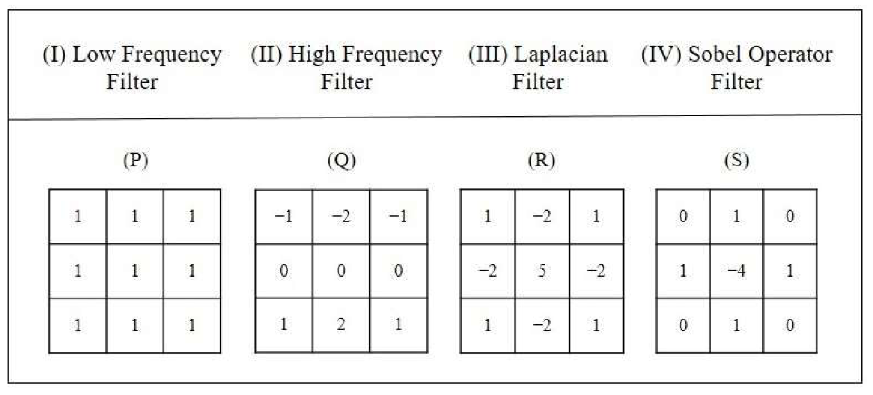
\includegraphics[width=0.9\columnwidth]{figs/fig_78.png}
    \label{fig:question78}
    \caption*{Figure.Q78}
\end{figure}

\hfill (GATE GE 2022)

\begin{enumerate}
\begin{multicols}{2}
    \item I - P and II - Q
    \item III - R and IV - S
    \item I - P and IV - Q
    \item II - R and III - S
\end{multicols}
\end{enumerate}

\item Band ratio in satellite images interpretation is applied to

\hfill (GATE GE 2022)

\begin{enumerate}
\begin{multicols}{2}
    \item enhance the spectral separation
    \item reduce the effects of topography
    \item enhance the effects of topography
    \item increase spatial differences between bands
\end{multicols}
\end{enumerate}

\item The decorrelation stretch enhances colour differences and removes inter-band \makebox[1cm]{\hrulefill}.

\hfill (GATE GE 2022)

\begin{enumerate}
\begin{multicols}{4}
    \item decorrelation
    \item contradiction
    \item correlation
    \item relationship
\end{multicols}
\end{enumerate}

\item The overall image classification accuracy (in percentage) calculated from the following error matrix is \makebox[1cm]{\hrulefill} (in integer).
\begin{figure}[H]
    \centering
    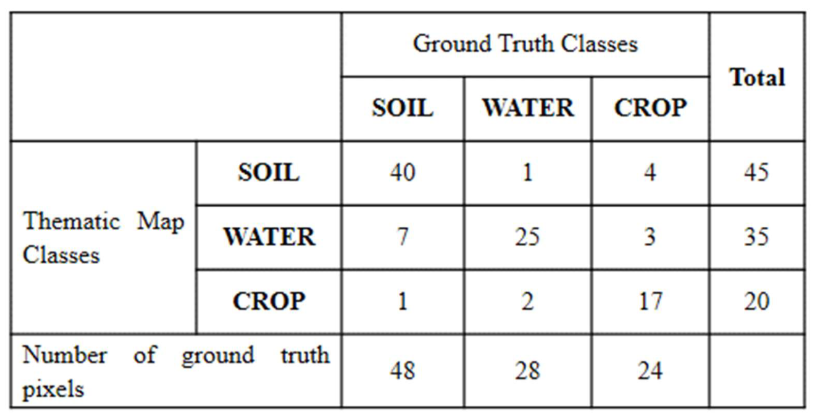
\includegraphics[width=0.8\columnwidth]{figs/fig_81.png}
    \label{fig:question81}
    \caption*{Figure.Q81}
\end{figure}

\hfill (GATE GE 2022)

\item Number of bytes required to store an 8-bit uncompressed image of size 512 $\times$ 512 pixels is \makebox[1cm]{\hrulefill} (in integer).

\hfill (GATE GE 2022)

\item The minimum and maximum Digital Number (DN) values of an image are 30 and 55, respectively. If the input DN value of a pixel is 35, the output DN value after linear contrast stretch of an 8-bit data is \makebox[1cm]{\hrulefill} (in integer).

\hfill (GATE GE 2022)

\item The FOV of a sensor (for a scene) placed at a nadir height of 6 km is 90°. The ground swath width of the scene is \makebox[1cm]{\hrulefill} km (in integer).

\hfill (GATE GE 2022)

\end{enumerate}

\end{document}